% Drawing 154/08-5 -- folder 154, batch 08, archive page 149 (PDF page 150).
% Transcription: croquis au crayon et à l'encre, sans texte : en haut, deux fuseaux allongés enfilés sur une droite ; au milieu, une droite brune passant par trois croisements en étoile, et un fuseau ; en bas, un arrangement de droites dont deux en tirets (vert et brun), trois croisements marqués ; un petit graphe en losange dans un ovale ; des segments isolés
% Kind: spindles strung on a line; line through three star crossings; arrangement with two dashed lines; small polygon. Method 2 (schematic redraw from the facsimile). Status: partial.
% Notes: Pencil and ink sketches without text over a printed accounting sheet (not reproduced), read from the page view: at the top, elongated spindles strung on a line; in the middle, a line passing through three star crossings, and a spindle; below, an arrangement of lines of which two dashed (green and brown), three crossings marked; a small polygon with marked vertices and further pencil spindles and segments. Lines placed approximately.
% Coordinates: 1 unit = 1 mm = 1/100 of the crop width (bbox in page fractions: [0.198, 0.13, 0.982, 0.502]).
% Redrawn by Claude (claude-opus-5-5), issue #73, 2026-11-07; not checked by a human; not compiled (no TeX in the session).
% Rights: reproduces part of the work -- behind RENDER_TRANSCRIPTS, never published by itself.
\documentclass[tikz,border=3pt]{standalone}
\usepackage{amsmath,amssymb}
\usetikzlibrary{patterns,arrows.meta}
\tikzset{Or/.style={orange!90!black}, Ye/.style={yellow!80!orange}, Lg/.style={green!60!black!70}, Dg/.style={green!45!black}, Br/.style={brown!80!black}, Rd/.style={red!85!black}, Bl/.style={blue!70!black}, Gy/.style={black!40}, pencil/.style={black!45}, struck/.style={black!35}, mark/.style={circle,draw,inner sep=1.3pt}, pt/.style={circle,fill,inner sep=0.9pt}, opt/.style={circle,draw,fill=white,inner sep=1.1pt}}
\begin{document}
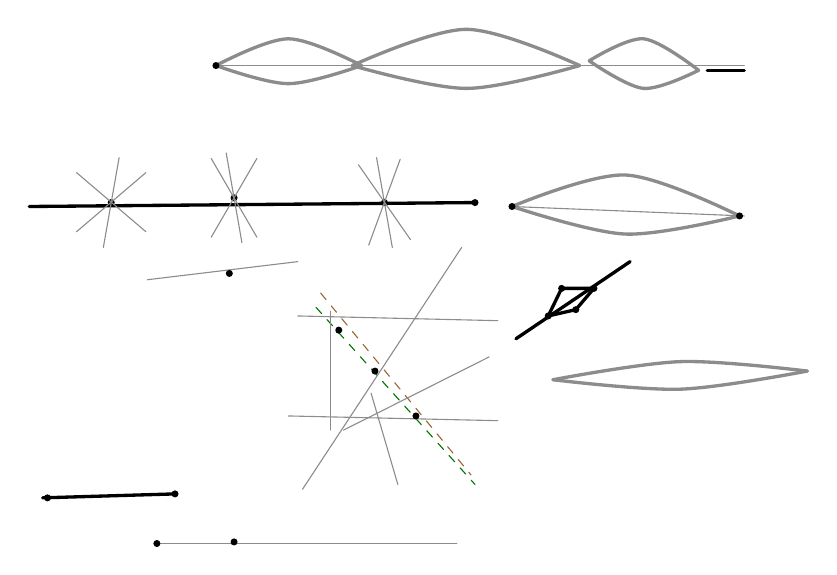
\begin{tikzpicture}[x=1mm,y=1mm,line cap=round,line join=round,font=\scriptsize]
\draw[pencil] (23.7,-4.6) -- (90.8,-4.6);
\draw[pencil,very thick] plot[smooth, tension=0.55] coordinates {(23.7,-4.6) (32.9,-1.2) (42.2,-4.6)};
\draw[pencil,very thick] plot[smooth, tension=0.55] coordinates {(23.7,-4.6) (32.9,-6.9) (42.2,-4.6)};
\draw[pencil,very thick] plot[smooth, tension=0.55] coordinates {(41,-4.6) (55.5,-0) (69.9,-4.6)};
\draw[pencil,very thick] plot[smooth, tension=0.55] coordinates {(41,-4.6) (55.5,-7.5) (69.9,-4.6)};
\draw[pencil,very thick] plot[smooth, tension=0.55] coordinates {(71.1,-4) (78,-1.2) (85,-5.2)};
\draw[pencil,very thick] plot[smooth, tension=0.55] coordinates {(71.1,-4) (78,-7.5) (85,-5.2)};
\node[pt] at (23.7,-4.6) {};
\draw[very thick] (86.1,-5.2) -- (90.8,-5.2);
\draw[very thick] (0,-22.5) -- (56.6,-22);
\node[pt] at (10.4,-22) {};
\node[pt] at (26,-21.4) {};
\node[pt] at (45.1,-22) {};
\node[pt] at (56.6,-22) {};
\draw[pencil] (6,-25.7) -- (14.8,-18.2);
\draw[pencil] (9.4,-27.7) -- (11.4,-16.3);
\draw[pencil] (14.8,-25.7) -- (6,-18.2);
\draw[pencil] (23.1,-26.4) -- (28.9,-16.4);
\draw[pencil] (27,-27.1) -- (25,-15.7);
\draw[pencil] (28.9,-26.4) -- (23.1,-16.4);
\draw[pencil] (43.1,-27.4) -- (47.1,-16.5);
\draw[pencil] (46.1,-27.7) -- (44.1,-16.3);
\draw[pencil] (48.4,-26.7) -- (41.8,-17.2);
\draw[pencil] (61.3,-22.5) -- (90.8,-23.7);
\draw[pencil,very thick] plot[smooth, tension=0.55] coordinates {(61.3,-22.5) (75.7,-18.5) (90.2,-23.7)};
\draw[pencil,very thick] plot[smooth, tension=0.55] coordinates {(61.3,-22.5) (75.7,-26) (90.2,-23.7)};
\node[pt] at (61.3,-22.5) {};
\node[pt] at (90.2,-23.7) {};
\draw[pencil] (15,-31.8) -- (34.1,-29.5);
\node[pt] at (25.4,-31) {};
\draw[Dg,dashed] (36.4,-35.3) -- (56.6,-57.8);
\draw[Br,dashed] (37,-33.5) -- (56.1,-56.6);
\draw[pencil] (34.1,-36.4) -- (59.5,-37);
\draw[pencil] (32.9,-49.1) -- (59.5,-49.7);
\draw[pencil] (38.2,-35.8) -- (38.2,-50.9);
\draw[pencil] (34.7,-58.4) -- (54.9,-27.7);
\draw[pencil] (39.9,-50.9) -- (58.4,-41.6);
\draw[pencil] (43.4,-46.2) -- (46.8,-57.8);
\node[pt] at (39.3,-38.2) {};
\node[pt] at (43.9,-43.4) {};
\node[pt] at (49.1,-49.1) {};
\draw[very thick] (61.8,-39.3) -- (76.3,-29.5);
\draw[very thick] (65.9,-36.4) -- (67.6,-32.9) -- (71.7,-32.9) -- (69.4,-35.6) -- cycle;
\node[pt] at (65.9,-36.4) {};
\node[pt] at (67.6,-32.9) {};
\node[pt] at (71.7,-32.9) {};
\node[pt] at (69.4,-35.6) {};
\draw[pencil,very thick] plot[smooth, tension=0.55] coordinates {(66.5,-44.5) (82.7,-42.2) (98.8,-43.4)};
\draw[pencil,very thick] plot[smooth, tension=0.55] coordinates {(66.5,-44.5) (82.7,-45.7) (98.8,-43.4)};
\draw[very thick] (1.7,-59.5) -- (18.5,-59);
\node[pt] at (2.3,-59.5) {};
\node[pt] at (18.5,-59) {};
\draw[pencil] (16.2,-65.3) -- (54.3,-65.3);
\node[pt] at (16.2,-65.3) {};
\node[pt] at (26,-65.1) {};
\end{tikzpicture}
\end{document}
